\newcommand{\sig}{\sigma}
\newcommand{\eps}{\epsilon}
\newcommand{\del}{\delta}
\newcommand{\ah}{\alpha}
\newcommand{\lam}{\lambda}
\newcommand{\gam}{\gamma}
\newcommand{\kap}{\kappa}
\newcommand{\rarr}{\rightarrow}
\newcommand{\larr}{\leftarrow}
\newcommand{\lrarr}{\Leftrightarrow}
\newcommand{\ol}{\overline}
\newcommand{\mbb}{\mathbb}
\newcommand{\contra}{\Rightarrow\Leftarrow}
% for cross product
\newcommand{\lc}{\langle} %<
\newcommand{\rc}{\rangle} %>
\newcommand{\pri}{^{'}} %'

%other shortcuts
\newcommand{\ben}{\begin{enumerate}}
\newcommand{\een}{\end{enumerate}}
\newcommand{\beq}{\begin{quote}}
\newcommand{\enq}{\end{quote}}
\newcommand{\hsone}{\hspace*{1cm}}
\newcommand{\hstwo}{\hspace*{2cm}}
% vision
\newcommand{\conv}{\convolution}
\newcommand{\Ix}{I_x}
\newcommand{\Iy}{I_y}
\newcommand{\Ixy}{I_{xy}}
% big 0
\newcommand{\cO}{\mathcal{O}}
% calc
\renewcommand{\vec}[1]{\boldsymbol{#1}}
% gradient
\newcommand{\grad}{\nabla}

\newcommand{\noi}{\noindent}
\parskip 5pt
\parindent 0pt

\documentclass[10pt,a4paper]{article}
\usepackage[letterpaper,hmargin=1.15in,vmargin=1.25in]{geometry} % full page dimensions
\usepackage{amsmath,amssymb,algorithmic,mathabx,hyperref,graphicx}
\begin{document}
\title{Image Segmentation CS828 Spring '12 Project 1\\ Nonliner Diffusion}
\author{Angjoo Kanazawa}
\maketitle

\section{Results}
\label{sec:results}

\subsection{Gaussian Smoothing}
\label{sec:gaussian-smoothing}
\begin{figure}[htb]
\centering
\subfloat[original]{\includegraphics[scale=0.5]{orig}}
\subfloat[noised]{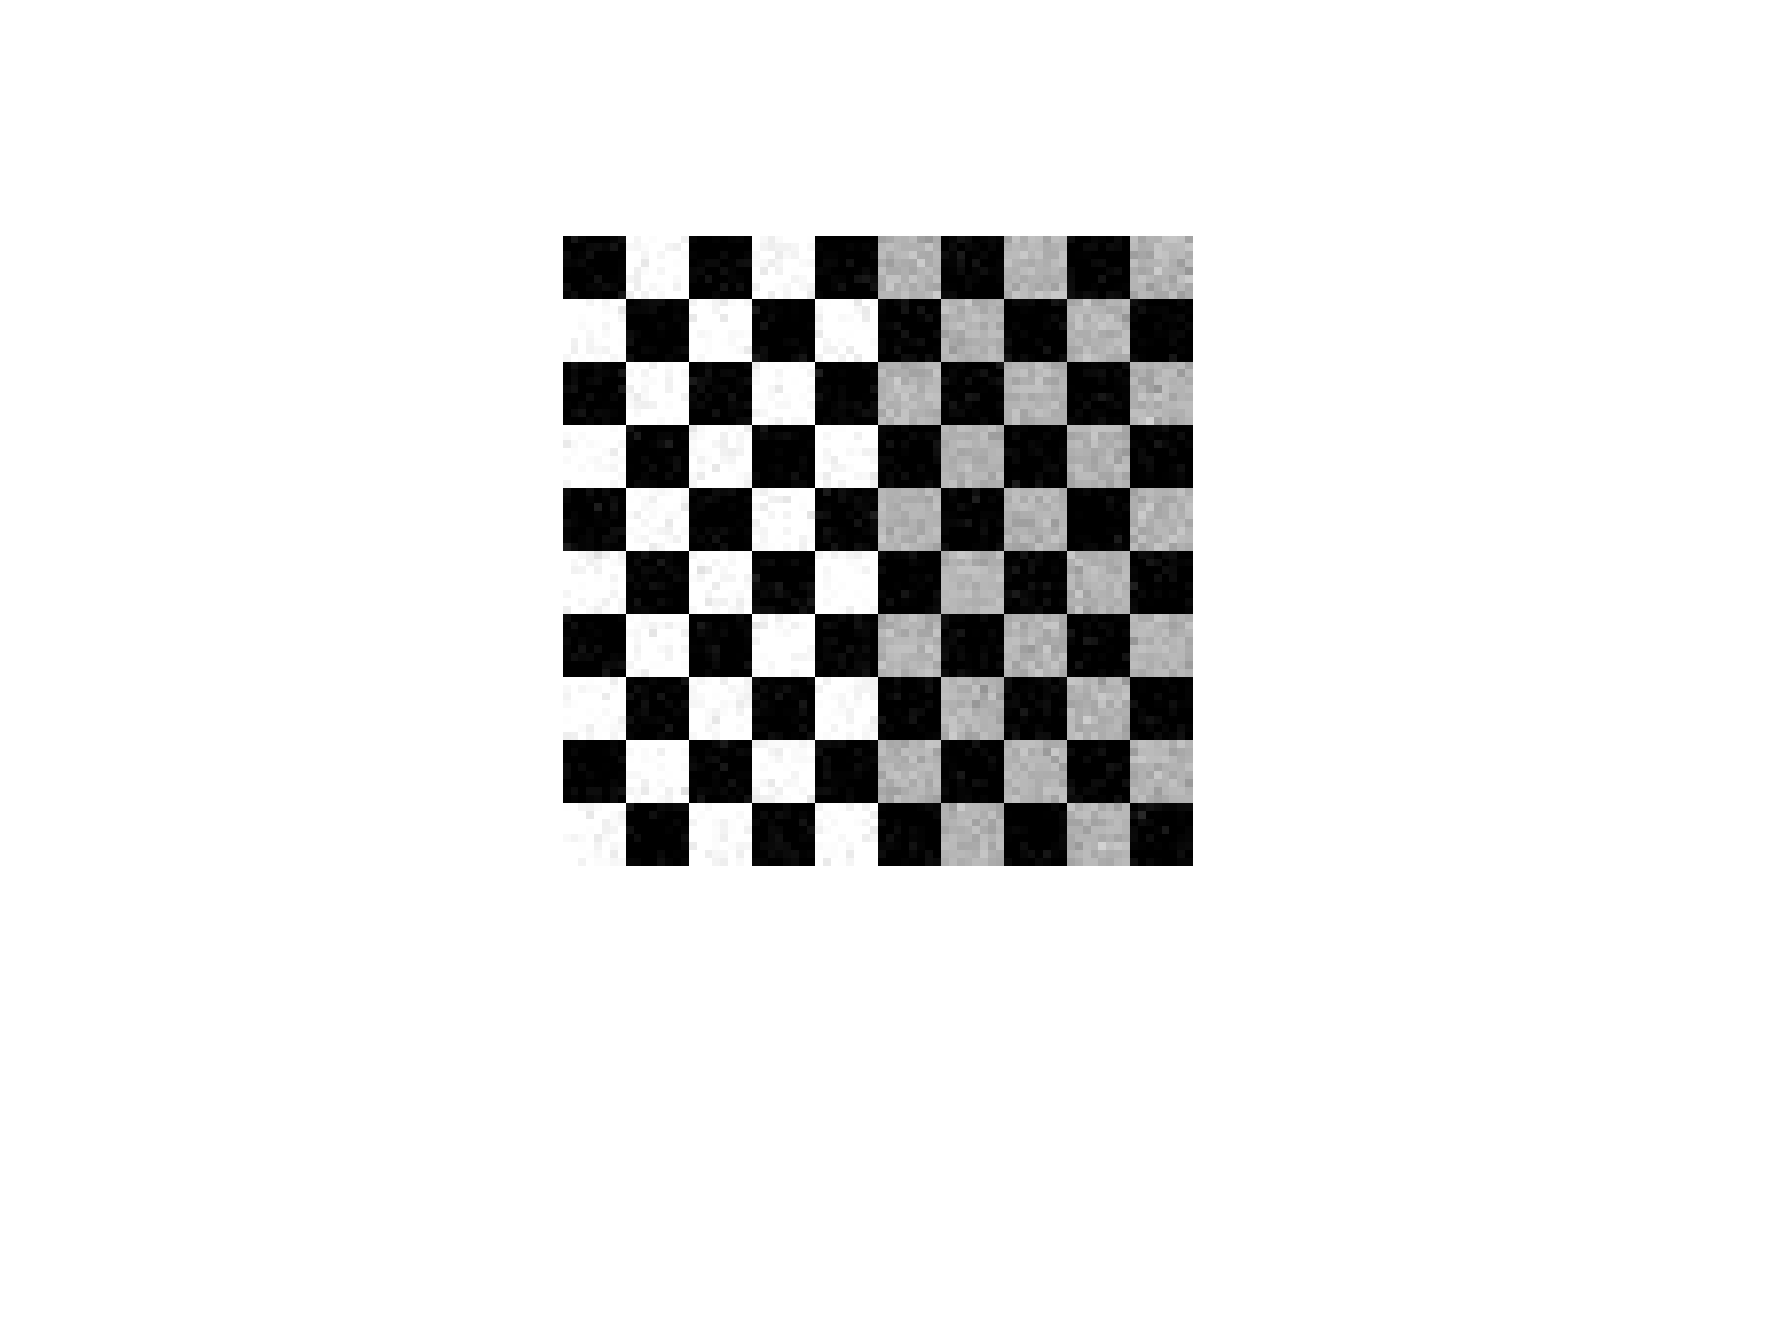
\includegraphics[scale=0.5]{noise}}
\subfloat[gaussian]{\includegraphics[scale=0.5]{gaussian}}
\caption{Original, noised, and Gaussian smoothing}
\end{figure}


\subsection{Perona-Malik, Anisotropic Nonlinear Diffusion (edge enhancing)}
\begin{figure}[htb]
\centering
\subfloat[Perona Malik]{\includegraphics[scale=0.5]{pm}}
\subfloat[Anisotropic Nonlinear Diffusion]{\includegraphics[scale=0.5]{nld}}
\caption{Perona Malik, Edge Enhancing Nonlinear Diffusion}
\end{figure}

\subsection{Non-local Means}
\label{sec:non-local-means}
\begin{figure}[htb]
\centering
\includegraphics[scale=0.5]{nlmeans}
\caption{non-local means}
\end{figure}

\section{Experimentation}
\label{sec:experimentation}


\pagebreak
\pagebreak

\end{document}
